\section{Testing}\label{Testing}
    [The testing setup and suite. The testing method and how we did the testing.]
    
    \subsection{Unit testing}\label{Unit testing}
    We decided quite early on that we wanted to do unit testing of every piece of code that we would produce, i.e. test driven development. The reason behind this choice is that we think this will result in better code quality along. The added bonus of easing integration testing, because we can easily discover if a new code addition will integrate with old code, is just icing on the cake. Also writing the tests first let us concentrate more on exactly what the methods should do instead of the content and how it should do it. One of the problems with test driven development however is, the possible bias that could occur, we could end up only satisfying the test and not the actual requirements. This could be countered to some extent by writing more comprehensive tests. Another positive point in favour of unit testing is the requirement we have which states that the product has to be written in Java(\ref{glossary:java}) where such test are easy to integrate and write using JUnit(\ref{glossary:junit}).

    \subsection{Integration testing}\label{Integration testing}
    For integration testing we decided that we wanted do automated system testing every other week in collaboration with code reviews. The procedure we are going to follow is coding new features in a separate branch. Once every other week the finished branches will have all their unit tests run through thoroughly followed by a code review of at least one person, then if the automated system tests are fully operational they will also be run to look for additional errors which the unit tests can not pick up. This point is quite likely to change in the future as a two week time interval might be to long given the short implementation period. The advantage of doing this integration testing is better overall code quality since we will test code before it is used by other parts of the system. Since we are also doing code review people will also gain experience with other parts of the system which they previously had not worked on, this will benefit everyone since knowledge about the system is shared and it will help in the eventuality of someone getting sick. The advantage of developing in separate branches is the reduced risk of polluting code other people are working on and a better separation of stable and unstable code.

    \subsection{System testing}\label{System testing}
    When it comes to system testing the customer was quite insistent that we test the product thoroughly in an emulated network situation. Since we had some, albeit little, experience with NS3(\ref{glossary:ns3}) we decided that we wanted to do the system testing on it. The advantage with that is that the customer had some already set up testing scenarios and helper scripts designed for NS3 which they offered us to use. This will greatly reduce the time we need for setting up the test suit and it will also gives us the ability to have automated test which we don’t have to monitor or interact with. Another added advantage is easy testing as we only have to start a script in order to run the whole suit, but that comes at the cost of actually setting up the whole thing. As of the midterm report we have set quite a lot of time aside in order for us to implement the proper NS3 support we need. To monitor what is happening under the test our applications will output all important information regarding what is going on, in addition to this we will have a packet sniffer(\ref{glossary:packet sniffer}) on each end which will capture network traffic. Using this information we should be able to tell a whole lot about what is going on in the network and we should be able to decide whether we have met the requirements or not.

    Bellow are some of the detailed test cases which we will automate on top of NS3. The testing it self will be automated, but in order to get some result from the test some human interaction is needed to interpret the output data.

    \begin{figure}[h]
        \centering
        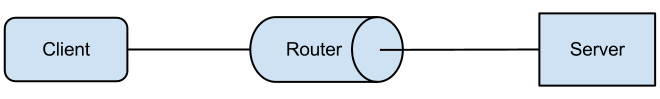
\includegraphics[scale=0.4]{Simplemessagesending}
        \caption{Simple message sending}
        \label{fig:Simple message sending}
    \end{figure}

    Simple message sending:\\
    In this test what we want to test is just the ability of the client and the ESB(\ref{glossary:esb}) to communicate. We want to see that the client is able to send messages(\ref{glossary:message}) to the server and get a response back. For monitoring purposes this test will rely on both applications to log their behavior. In order for us to give this test the green light we must see a message going out from the client then passing through the ESB to GlassFish(\ref{glossary:glassfish}). Then finally a reply should be sent back from GlassFish to the ESB and then to the client.

    Setting Quality of Service(QoS):\\
    In this test what we want to test is the client and the ESB’s ability to set the DiffServ(\ref{glossary:diffserv}) field in the IP header(\ref{glossary:ip header}). The first requirement in this test is that the test “Simple message sending” has been passed. For this test to be considered a success the client have to send a message to the ESB which is then sent back containing the DiffServ value in an SOAP header. The ESB must at this point have set the DiffServ value in the IP header. Then the client should use a service on GlassFish, but this time the IP header must contain the correct DiffServ value. In order to monitor this test only a packet sniffer located on the client and ESB side needs to be used. The packets must then be examined and the correct DiffServ value must be present in the IP header of all packets except the first one going out from the client.

    \begin{figure}[h]
        \centering
        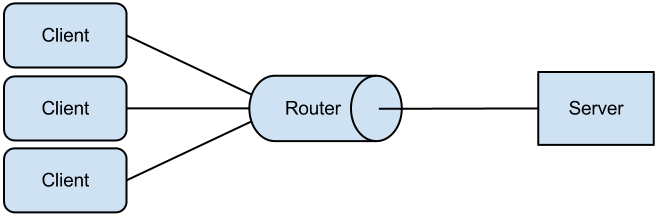
\includegraphics[scale=0.4]{3Clientmessagesending}
        \caption{3 client message sending}
        \label{fig:3 client message sending}
    \end{figure}
    
    Prioritizing messages:
    In this test we want to test the ESB’s ability to prioritize messages. The scenario will be set up such that two clients will send lots of messages trying to flood the capacity of the server. All of these messages should have the same priority, but intermittent the third client with the higher priority should send some messages. What we are looking for is that these higher priority messages should be sent out from the ESB ahead of lower priority and if necessary it have to stop some already sending messages. For this test to be successful we must see some lower priority messages being preempted or held back. To do this the log file of the ESB has to be studied and there should be some clear indications of one of the previous requirements.

    Changing DiffServ value:\\
    In this test what we want to check is the ESB’s ability to change DiffServ value after a reconfiguration. The test and the result can be examined and performed the same way as “Setting Quality of Service(QoS)”, but the difference this time is that the test have to be run twice one where the configuration has one DiffServ value and a second run where the DiffServ value has a different value. To evaluate this test to true one would have to examine the resulting pcap(\ref{glossary:pcap}) files on the server side and check each run to see if the two tries have different DiffServ values.

    \begin{figure}[h]
        \centering
        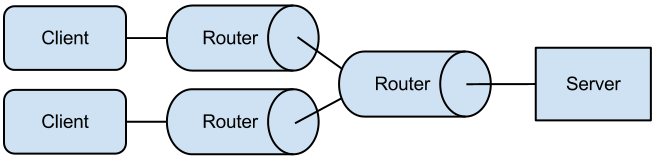
\includegraphics[scale=0.4]{2Clientdifferentpathsmessagesending}
        \caption{2 Clients different paths message sending}
        \label{fig:2 Clients different paths message sending}
    \end{figure}
    
    Multipath server routing:\\
    In this test we want to look at the ESB’s capabilities to talk to the MS(\ref{glossary:ms}) and understand the routing result. From the MS the ESB should get some routing information about the topology of the network. As you can see in \ref{3 client message sending} if the link between the server and the first router is not the limiting factor the two clients should not get in each others way. Therefor since we get the information about the last router from the MS the ESB should understand that there is no problem and should not preempt any messages. To check if this is actually the case the ESB should not after some time preempt any messages, the ESB will need some time to adjust as it does not get the full picture of the network topology, but after this time no messages should be dropped from the ESB’s side.

    \begin{figure}[h]
        \centering
        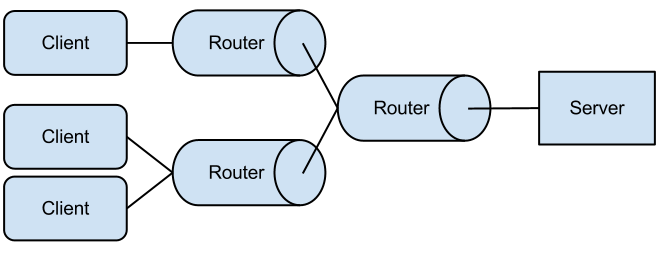
\includegraphics[scale=0.4]{3Clientswheretwoarecompeting}
        \caption{3 clients where two are competing}
        \label{fig:3 clients where two are competing}
    \end{figure}

    Competing clients in a multipath environment:\\
    This test is a compilation of the tests “Multipath server routing” and “Prioritizing messages”. For this test what we want to see is that the ESB is smart enough that it only preempts the messages going to one of the competing clients. As you can see in the figure \ref{3 clients two competing} there is one client which should not affect either of the two others if the link between the server and the first router is not a bottleneck. This should allow this client to receive messages even though the two other clients are competing for scarce resources. To check that this test is successful, a combination of the clients log files and the server log files will have to be used. If most(over 96\%) of the messages arrive at the higher priority client and the third client is not affected then this test is successful.

    Competing clients in a low bandwidth scenario:\\
    In this test we want to test that the ESB can manage to prioritize messages in a network with a joint bottleneck, but with different endpoints. In the figure \ref{3 clients two competing} if the link between the server and the first router is the bottleneck then the ESB should after a small initialisation understand that it has to preempt messages going out to all clients in order for a higher priority client to get the service it is supposed to get. The scenario will be set up in such a way that one of the two competing clients will have higher priority than the two others, the two lower priority clients should then send a steady stream of messages which should fill the bottleneck link. The third client should then start sending some messages which must now fill the entire bottleneck link and creating a situation where the ESB has to hold back or preempt messages going to either of the two other clients. As before a combination of the ESB and the clients log files have to be examined.
